\section{Configuration} \label{sec:configuration}
\noindent
In KitFox, a processor is represented as the hierarchy of \emph{pseudo components}.
Pseudo components are abstract units for which library models estimate physical phenomena.
Different physical properties are characterized at different levels of processor abstraction.
For instance, power is characterized at microarchitecture or circuit-level components using architectural activity counts.
Temperature is calculated at the package level, based on power distribution on the die.
Thus, pseudo components can represent different levels of processor abstraction, depending on which library models they are associated with and which physical properties are characterized.
A pseudo component may represent a microarchitectural component when an energy library model is associated with it to calculate power or energy dissipation.
Or it may be a processor package if a thermal library model is attached.
The pseudo component hierarchy can be flexibly composed to simulation different processor designs.
There is no inherent restriction on the number of levels in the pseudo component tree, and each pseudo component can have as many sub-components as necessary.
Figure \ref{fig:kitfox_hierarchy} illustrates an example of how KitFox framework serves to interface pseudo components and libraries to simulate a processor design. 
The simulated microarchitecture is decomposed into basic components (shown as ``sources'' in the figure), where power is estimated with energy library models.
Each energy library may derive a different sub-class tool, and it enables choosing the most appropriate model for different microarchitectural components.
Pseudo components can be grouped into another upper-level pseudo component (shown as ``floorplans'' in the figure) depending on their microarchitectural and technological similarities (e.g., core, memory).
Higher-level components may represent larger processor units such as cores or regions on the die.
The root component in the example represents the package and is linked to a thermal library model.
It can designate any descendant components in the tree as its constituent floorplans.
Some intermediate components without linked libraries can also be created for the convenience of processor description or data collection.
Every pseudo component includes data queues to store computed results of library models and shared data (e.g., voltage, frequency) for cross-referencing between pseudo components.

\begin{figure}[h]
\centering
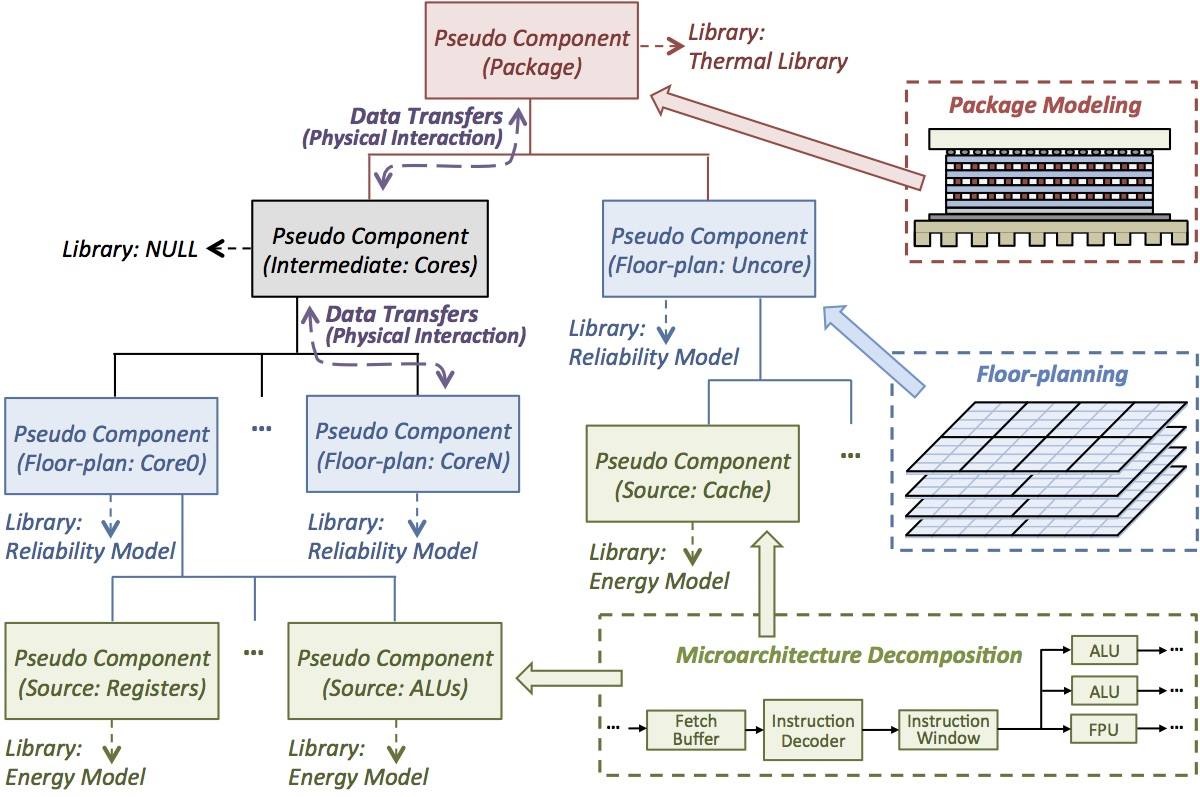
\includegraphics[width=0.6 \textwidth]{figures/kitfox_hierarchy.jpg}
\caption{A processor is represented as the \emph{pseudo component hierarchy} in KitFox framework. Pseudo components are physically defined units where associated libraries estimate physical phenomena. Physical interactions are emulated by transferring data between the data queues of pseudo components.}
\label{fig:kitfox_hierarchy}
\end{figure}

\subsection{Single Component Example} \label{subsec:single_component}
\noindent
The following shows an example of defining a pseudo component in the input configuration file. 
To define a pseudo component, it starts with the setting $|component|$.
In this example, a pseudo component $|package|$ is created. 
It has temperature and power data queues, each with a single entry; detailed discussion about the queue management will be covered later in the document (Section \ref{sec:data_queues}).
$|library|$ defines the parameters of the physical model associated with the $|package|$.
3D-ICE is used for package thermal model in this example, and transient simulation mode is used.
An example configuration to define 3D-ICE model can be found in $|config/3dice.config}|$ with 3D-stacked layers and a micro-channel model.
Similarly, refer to $|config|$ directory or Appendix to find how to use individual models integrated in KitFox.

{
\fontsize{10pt}{11pt}\selectfont
\begin{alltt}
component: \{
    package: \{ // package component
        data_queue = ["KITFOX_DATA_TEMPERATURE", "KITFOX_DATA_POWER"];
        queue_size = 1;
        /* Parameters of the physical model */
        library: \{
            model = "3d-ice"; // Use 3D-ICE for package thermal model
            thermal_analysis_type = "transient";
            grid_rows = 64;
            grid_columns = 64;
            ... // And more 3D-ICE parameters to be defined
        \};
    \};
\};
\end{alltt}
}

\subsection{Multi-Level Components, Multiple Models, and Shared Parameters} \label{subsec:multilevel_components}
\noindent
Pseudo components can be recursively created to construct multiple levels of pseudo component hierarchy. 
$|component|$ within the $|package|$ lists the sub-components whose name paths are delimited by dots, $|package.cores.core0|$ for example.
In the example below, $|package.cores|$ is a dummy component that is not associated with any physical models.
Dummy components can be created for better hierarchical processor description or data management purpose that will be described later in the document (Section \ref{sec:data_queues}).
$|package.cores.core0|$ and $|package.cores.core1|$ are the floorplans of the thermal library associated with the root component $|package|$.
The floorplans are associated with the failure models for reliability modeling.
In $|package.cores.core0|$, $|voltage|$ variable is defined as 0.9V, but $|package.cores.core1|$ does not define the $|voltage|$ that is necessary for the failure model.
If a required variable is not defined, KitFox recursively searches the parameter in the components along the path to the root when parsing the input configuration file.
In this example, $|voltage|$ is defined in the root component $|package|$, and therefore $|package.cores.core1|$ uses 1.0V as the initial voltage input.
The recursive search of parameters avoids defining the same parameter of the same value multiple times across pseudo components and simplifies the configuration by defining the common parameters in the parent components. 
Hence, the parameters common to multiple, distinct physical models can be defined only once and shared.

{
\fontsize{10pt}{11pt}\selectfont
\begin{alltt}
component: \{
    package: \{ // package component
        /* Parameters of the physical model */
        library: \{
            model = "3d-ice";
            ... // And more 3D-ICE parameters to be defined
            
            /* Common library parameters under the package */
            clock_frequency = 2.0e9; // 2GHz clock frequency
            voltage = 1.0; // 1V supply voltage
            
            floorplan = [
                "package.cores.core0",
                "package.cores.core1",
                "package.uncore.l2cache"
            ];
        \};
        component: \{
           cores: \{ // package.cores component
                library: \{
                    model = "none"; // No physical model is associated.
                \};
                component: \{
                   core0: \{ // package.cores.core0 component 
                        library: \{
                            model = "failure"; // Use Failure model for reliability
                            voltage = 0.9; // Overwritten supply voltage
                            ... // And more Failure model parameters to be defined
                        \};
                    \};
                core1: \{ // package.cores.core1 component
                        library: \{
                            model = "failure"; // Use Failure model for reliability
                            ... // And more Failure model parameters to be defined
                        \};
                    \};
                \};
            \};
            uncore: \{ // package.uncore component
                library: \{
                    model = "failure"; // Use Failure model for reliability
                    ... // And more Failure model parameters to be defined
                \};
                component: \{
                   l2cache: \{ // package.uncore.l2cache component
                        library: \{
                            model = "mcpat"; // Use McPAT for L2\$ power model
                            energy_model = "cache"; // Use cache model in McPAT
                            line_size = 64; // Cache line size
                            ... // And more McPAT parameters to be defined
                        \};
                    \};
                \};
            \};
        \};
    \};
\};
\end{alltt}
}

\noindent
The pseudo components created in KitFox can be identified in two ways; string \emph{name} and integer \emph{ID}.
Name is the component path such as $|package.cores.core0|$, and ID is a sequentially assigned integer number by KitFox when creating the pseudo components.
KitFox provides functions to acquire the pseudo component ID with the name, or the name can be retrieved with the ID.
Detailed will be covered in the document (Section \ref{sec:list_of_api_functions} or \ref{sec:data_queues}).

